%% chapter11_slides.tex
%% Chapter 11: Delivering Letters
%% Nature Inspired Optimisation for Delivery Problems (2022)
%% Self-contained lecture slides — reader-friendly format
%%
%% Compile: pdflatex -interaction=nonstopmode chapter11_slides.tex  (run twice)

\documentclass[aspectratio=169,10pt]{beamer}

\usetheme{Madrid}
\usecolortheme{seahorse}

\usepackage{amsmath,amssymb}
\usepackage{graphicx}
\usepackage{booktabs}
\usepackage{array}
\usepackage{xcolor}
\usepackage{listings}
\usepackage{microtype}
\usepackage{tikz}
\usetikzlibrary{shapes.geometric,arrows.meta,positioning,fit}
\usepackage[T1]{fontenc}
\usepackage{hyperref}
\hypersetup{colorlinks=true,linkcolor=blue,urlcolor=blue,pdfencoding=auto}

\graphicspath{{figures/}}

%% Listings style for Java / pseudocode
\lstdefinestyle{java}{
  language=Java,
  basicstyle=\ttfamily\scriptsize,
  numbers=left,
  numberstyle=\tiny\color{gray},
  stepnumber=1,
  frame=single,
  backgroundcolor=\color{gray!7},
  keywordstyle=\color{blue!70!black}\bfseries,
  commentstyle=\color{green!50!black}\itshape,
  stringstyle=\color{red!60!black},
  breaklines=true,
  showstringspaces=false,
  tabsize=2,
  xleftmargin=1.5em,
  framexleftmargin=1.5em,
}

%% Listings style for pseudocode
\lstdefinestyle{pseudo}{
  basicstyle=\ttfamily\scriptsize,
  numbers=left,
  numberstyle=\tiny\color{gray},
  frame=single,
  backgroundcolor=\color{gray!7},
  keywordstyle=\color{blue!70!black}\bfseries,
  commentstyle=\color{green!50!black}\itshape,
  breaklines=true,
  tabsize=2,
  xleftmargin=1.5em,
  framexleftmargin=1.5em,
  morekeywords={Procedure,EndProcedure,if,then,else,while,do,return,Return,true,false,and,not},
}

\setbeamertemplate{footline}[frame number]
\setbeamertemplate{navigation symbols}{}

%% ─────────────────────────────────────────────────────────────────────────────
\title[Chapter 11: Delivering Letters]{%
  Chapter 11: Delivering Letters\\[4pt]
  \normalsize Street-Based Routing with Evolutionary Algorithms}
\subtitle{Nature Inspired Optimisation for Delivery Problems (2022)}
\author{N.\ Urquhart}
\date{Lecture Notes --- Self-Contained Reader Edition}

%% ─────────────────────────────────────────────────────────────────────────────
\begin{document}

\begin{frame}
  \titlepage
\end{frame}

%% ─────────────────────────────────────────────────────────────────────────────
\begin{frame}[allowframebreaks]{Table of Contents}
  \tableofcontents
\end{frame}

%% =============================================================================
\section{11.1 Introduction}
%% =============================================================================

\begin{frame}[allowframebreaks]{11.1 Introduction -- The Postal Delivery Problem}

  Postal workers, charity collectors, census takers, and political canvassers all
  share a common challenge: they must visit every house in a given area while
  walking as short a total distance as possible.
  This is an example of a \textbf{house-to-house delivery} routing problem in
  an urban setting.

  \begin{block}{Problem Statement}
    Given a set of delivery addresses distributed across a network of streets,
    find the shortest walking route that visits every address exactly once,
    starting and ending at a fixed depot (e.g.\ a postal sorting office or
    a parked van).
  \end{block}

  \textbf{Why not just use the Travelling Salesperson Problem (TSP)?}
  The natural first instinct is to model each delivery address as a city in a
  TSP.  For $n$ addresses, the TSP has a solution space of $n!/2$ possible
  routes (dividing by 2 because the route can be traversed in either direction,
  giving the same total distance).  For just 50 addresses this is already
  $50!/2 \approx 1.5 \times 10^{63}$, a number far beyond exhaustive search.
  For hundreds of addresses --- which is typical for a single postal walk ---
  the TSP becomes computationally intractable.

  \begin{alertblock}{Key Challenge}
    The TSP scales poorly because it treats every single address as an
    independent entity.  It ignores the fact that in urban environments,
    addresses cluster naturally into streets, and streets connect at junctions.
    This structure can be exploited to reduce the search space dramatically.
  \end{alertblock}

  \framebreak

  \textbf{Urban structure offers an opportunity.}
  Within a city, individual addresses group together in a very regular way:

  \begin{itemize}
    \item Addresses sit on one or both sides of a \emph{street section}
          --- the segment of a street between two consecutive junctions.
    \item Street sections connect to each other at \emph{junctions}
          (corners, T-junctions, roundabouts, etc.).
    \item A delivery worker walking down a street section will naturally deliver
          to all addresses on that section before moving to the next.
  \end{itemize}

  The figure below shows an extract from a real city map where addresses
  have been grouped into street sections.  Red squares mark individual
  delivery addresses; orange circles mark junctions.

  \begin{center}
    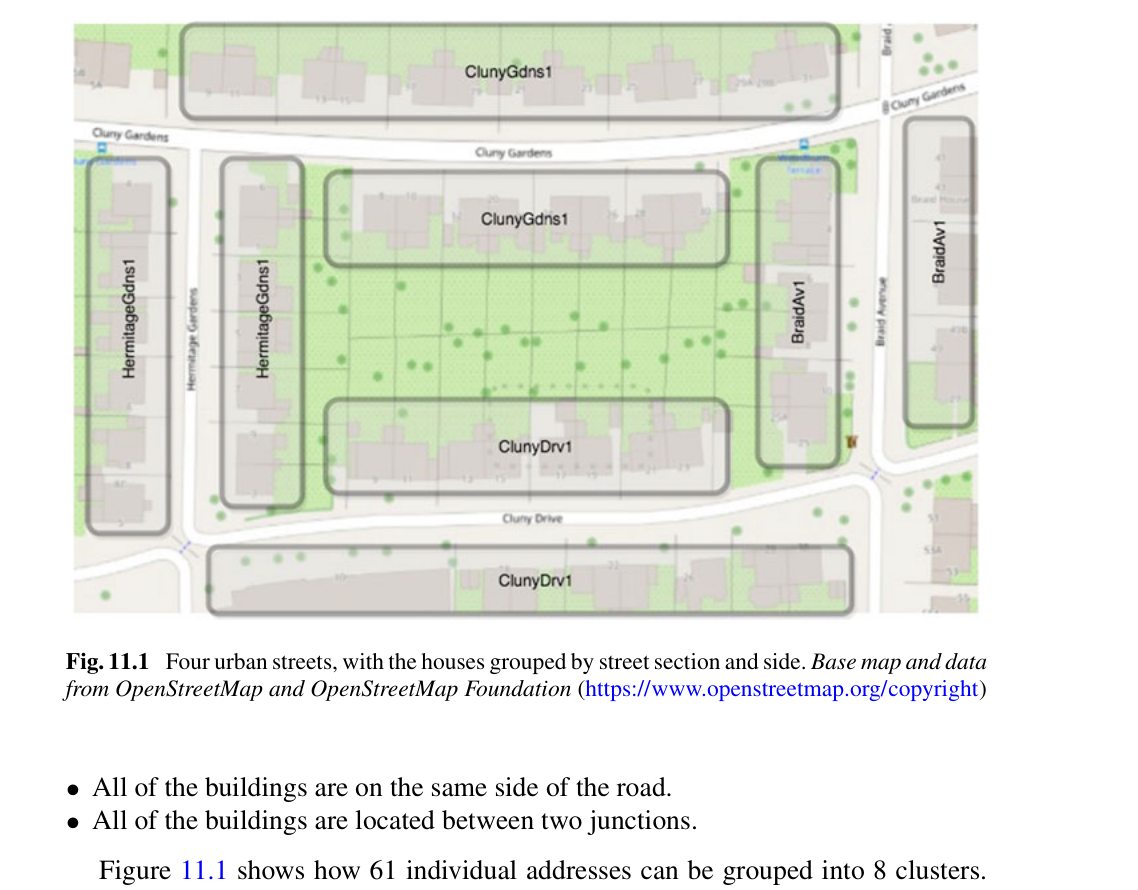
\includegraphics[width=0.70\linewidth]{fig_book_street_map.png}
  \end{center}

  \framebreak

  \textbf{Two grouping criteria} determine which addresses form a street section:
  \begin{enumerate}
    \item All of the buildings are on the \textbf{same side} of the road; and
    \item All of the buildings lie \textbf{between the same two junctions}.
  \end{enumerate}

  For example, the section labelled \texttt{ClunyGdns1} contains all the
  odd-numbered houses on Cluni Gardens that fall between junction~J1 and
  junction~J2.

  \begin{alertblock}{Key Insight}
    Once we accept that deliveries to adjacent addresses should always stay
    together (which is physically natural --- why walk away from a house you
    need to deliver to?), we can group them into street sections and treat
    each section as a single unit.  The search space drops from $n!$ (one
    permutation per individual address) to $s!$, where $s$ is the number of
    sections and $s \ll n$.
  \end{alertblock}

  \textbf{Historical context.}  The Street Based Routing (SBR) method
  described in this chapter was originally introduced in Urquhart et al.\
  (2001) as part of a PhD thesis at Edinburgh Napier University.  It combines
  a domain-specific chromosome \emph{representation} with a custom
  \emph{decoder} so that an Evolutionary Algorithm (EA) can search the reduced
  street-section space efficiently.

\end{frame}

%% =============================================================================
\section{11.2 Street Based Routing}
%% =============================================================================

\begin{frame}[allowframebreaks]{11.2 Street Based Routing -- Representation}

  The central idea of SBR is a \textbf{chromosome} (the EA's encoding of a
  candidate solution) whose genes are \emph{street sections} rather than
  individual addresses.  Each gene is simply the name (or identifier) of a
  street section.

  \begin{block}{Definition: SBR Chromosome}
    An SBR chromosome is an ordered list of street-section identifiers.
    The order of genes in the chromosome determines the order in which the
    delivery worker visits the street sections.  Each gene is expanded into
    its full list of individual delivery addresses during \emph{decoding}.
  \end{block}

  A worked example illustrates this well.  Suppose the delivery area contains
  five street sections: \texttt{ClunyGdns1}, \texttt{ClunyDrv1},
  \texttt{BraidAv1}, \texttt{HermitageGdns1}, and their double-sided
  counterparts.  A valid chromosome (as shown in Table~11.1 of the book) is:

  \begin{center}
    \begin{tabular}{|c|c|c|c|c|c|c|c|}
      \hline
      \texttt{ClunyGdns1} & \texttt{ClunyDrv1} & \texttt{ClunyDrv1} &
      \texttt{BraidAv1} & \texttt{HermGdns1} & \texttt{HermGdns1} &
      \texttt{BraidAv1} & \texttt{ClunyGdns1} \\
      \hline
      Gene 1 & Gene 2 & Gene 3 & Gene 4 & Gene 5 & Gene 6 & Gene 7 & Gene 8 \\
      \hline
    \end{tabular}
  \end{center}

  Notice that \texttt{ClunyDrv1} and \texttt{HermitageGdns1} each appear
  \emph{twice} in the chromosome.  This is because these sections have houses
  on \textbf{both sides} of the road.  When a section appears twice, the
  decoder treats the two appearances as two separate operations: one for each
  side of the street.  When the two appearances are \emph{adjacent} in the
  chromosome, the decoder delivers to both sides in a single pass (a U-turn
  at one end).  When they are \emph{separated}, the decoder delivers to each
  side on two separate visits.

  \framebreak

  \begin{center}
    
\includegraphics[width=0.80\linewidth]{fig_chromosome.pdf}
  \end{center}

  The figure above shows the chromosome as a sequence of colour-coded boxes.
  Same-coloured pairs (connected by arrows) are the two genes for a
  double-sided street section.  Same colour means same street section;
  different positions in the sequence mean different visits.

  \begin{alertblock}{Why Pairs for Double-Sided Streets?}
    A double-sided street section has two distinct sets of addresses ---
    one on the left footpath and one on the right.  The delivery worker can
    choose to deliver both sides in one sweep (U-turn pattern) or visit them
    on separate occasions.  The SBR chromosome captures this naturally:
    two identical consecutive genes = one combined sweep;
    two identical non-adjacent genes = two separate visits.
  \end{alertblock}

  \framebreak

  \textbf{Three things the decoder must determine for each section:}

  \begin{enumerate}
    \item \textbf{The starting junction}: which end of the section to enter
          from.  This is the junction closest to the \emph{previous delivery}
          in the route (using nearest-neighbour logic).
    \item \textbf{The ending junction}: which end to exit from.  This is the
          junction closest to the \emph{next gene's} section.
    \item \textbf{Single-sided or double-sided}: whether to deliver only one
          side, or both sides in a single sweep (determined by whether the gene
          appears adjacent to its partner or not).
  \end{enumerate}

  A powerful \textbf{pre-processing optimisation} follows from this structure.
  Because we know which addresses belong to each section, and which junctions
  bound each section, we can \emph{pre-compute} the optimal ordering of
  addresses for all three patterns (one side, both sides, cross-over) at
  startup.  These cached orderings are reused every time the decoder visits
  that section, avoiding repeated nearest-neighbour calculations during the EA
  evaluation loop.

\end{frame}

\begin{frame}[allowframebreaks]{11.2 Street Based Routing -- Delivery Patterns}

  When the decoder processes a gene, it selects one of several
  \textbf{delivery patterns} depending on the start junction, end junction,
  and whether the section is being delivered as single-sided or double-sided.
  The figure below illustrates the three main patterns.

  \begin{center}
    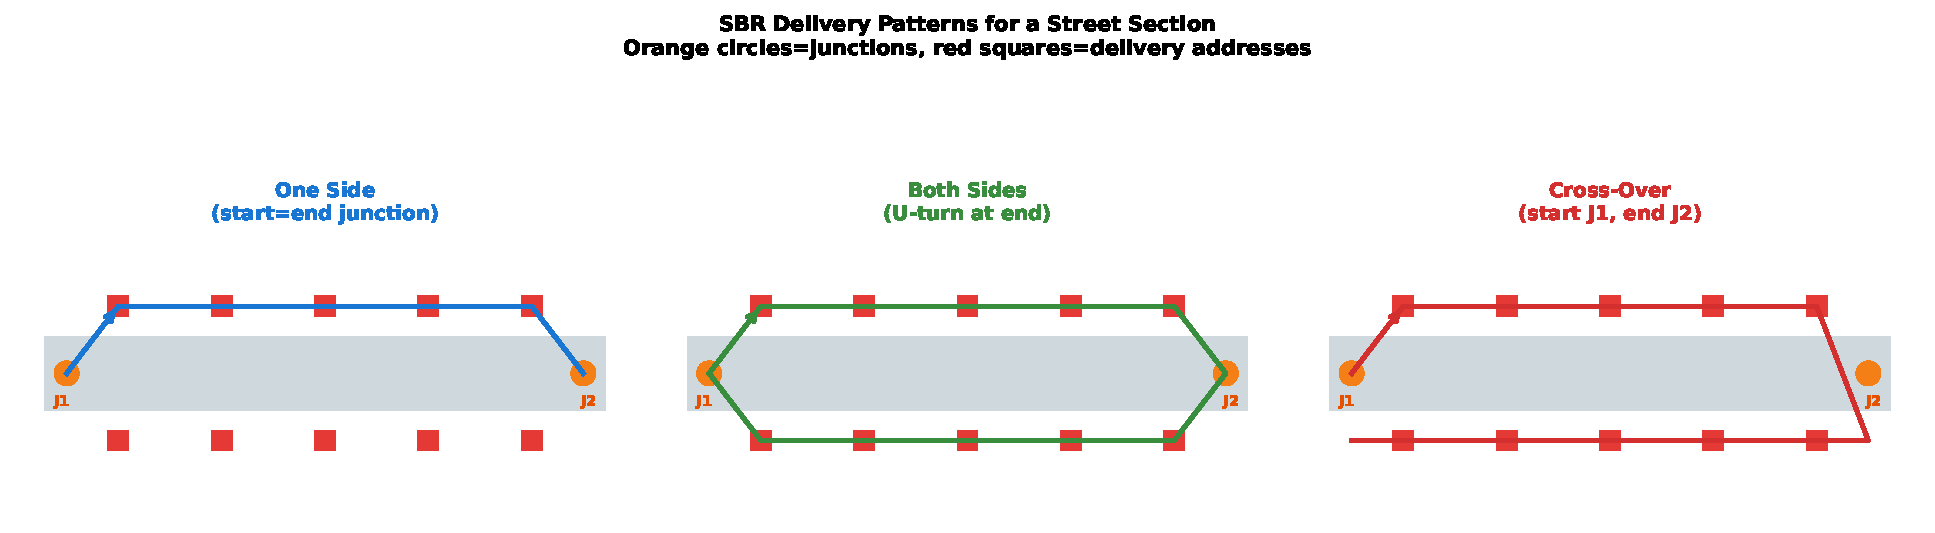
\includegraphics[width=0.90\linewidth]{fig_delivery_patterns.pdf}
  \end{center}

  \textbf{Pattern 1 --- One side, same junction (straight walk):}
  The worker enters the section from junction~J1 (the nearest junction to the
  previous delivery), walks along one side of the street delivering to all
  houses, and exits back through J1.  This happens when J1 is also the
  closest junction to the \emph{next} section.

  \textbf{Pattern 2 --- Both sides, U-turn at far end:}
  The worker enters from J1, delivers all houses on side~1 while walking to
  J2, then crosses the road and delivers all houses on side~2 while walking
  back to J1.  This is the most efficient pattern when both sides are being
  delivered in one combined sweep.

  \textbf{Pattern 3 --- Cross-over (opposite junctions):}
  The worker enters from J1 but must exit at J2 (because J2 is closer to the
  next section).  In this case both sides are delivered in the direction of
  travel, and the worker exits at J2 having crossed from one side to the other.

  \framebreak

  The book shows the actual map-based decoding step-by-step in Fig.~11.2.
  Below is the crop from the book showing how the first two genes of the
  example chromosome are decoded onto the real street layout:

  \begin{center}
    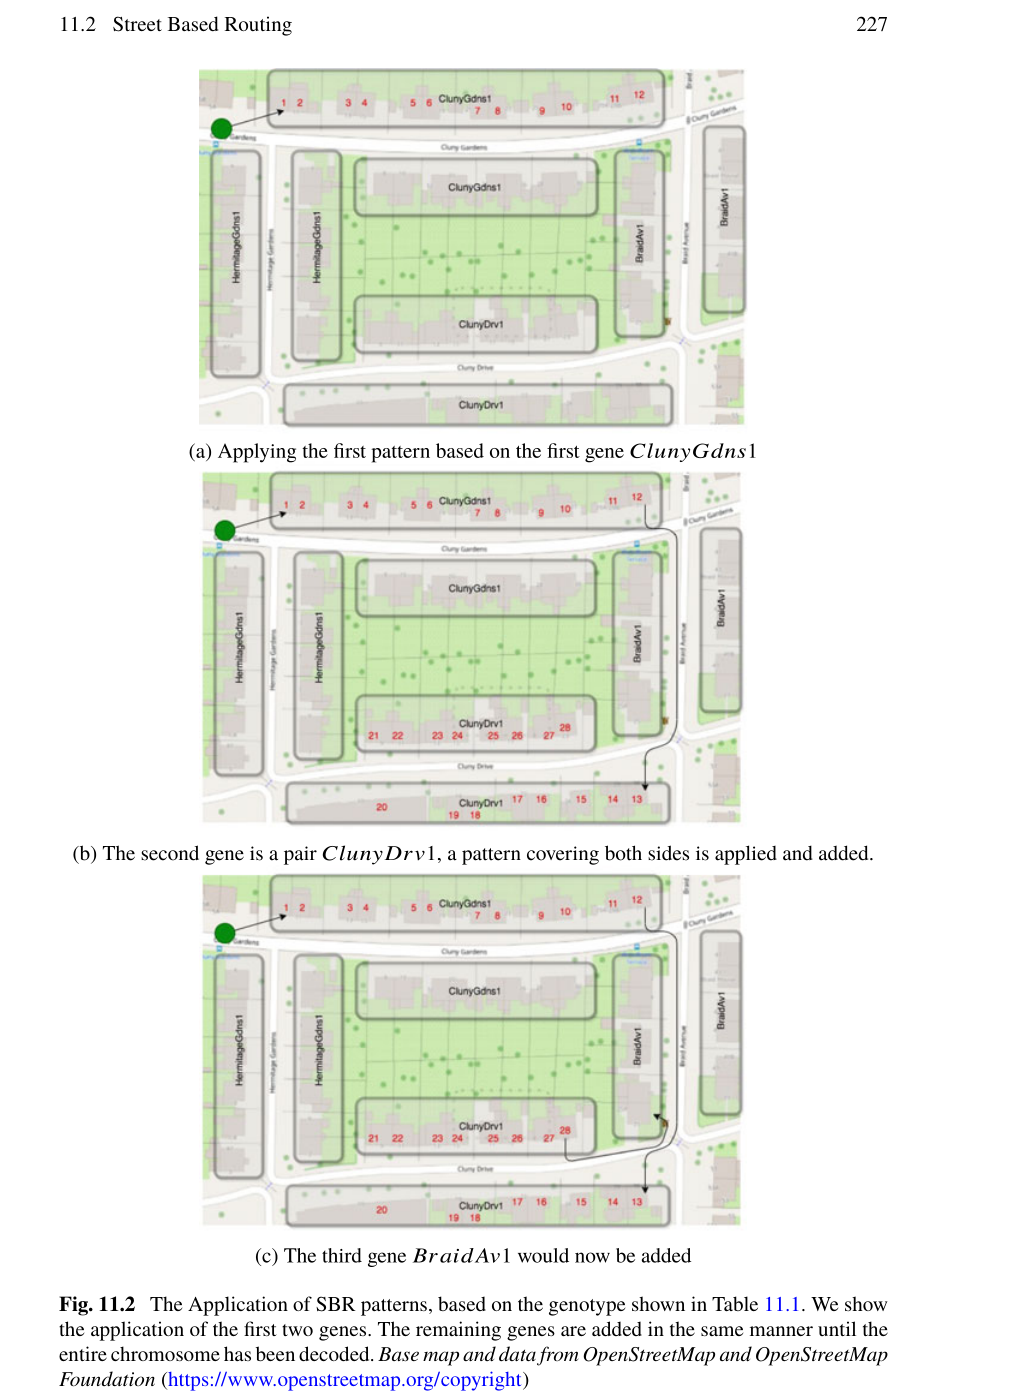
\includegraphics[width=0.82\linewidth]{fig_book_sbr_decode.png}
  \end{center}

  \begin{block}{Table 11.2 --- Examples of Delivery Patterns}
    \begin{center}
    \begin{tabular}{lll}
      \toprule
      Gene pair type & Start junction & Pattern applied \\
      \midrule
      Single gene (one side) & Nearest to prev.\ delivery & One-side walk \\
      Adjacent pair (both sides) & Nearest to prev.\ delivery & U-turn sweep \\
      Non-adjacent pair & Nearest to prev.\ delivery & Cross-over or separate \\
      \bottomrule
    \end{tabular}
    \end{center}
  \end{block}

\end{frame}

\begin{frame}[allowframebreaks]{11.2 Street Based Routing -- Decoding Algorithm}

  The complete decoding procedure (Algorithm~22) translates a genotype (list
  of street-section genes) into a \textbf{phenotype} (the actual walking route
  with all individual delivery addresses).

  \begin{block}{Algorithm 22: SBR Decoding}
    \textbf{Input:} \texttt{genotype} (ordered list of street sections),
    \texttt{problem} (start/end depot, all addresses)\\
    \textbf{Output:} Total walking distance of the decoded route
  \end{block}

  \textbf{Reading the algorithm step by step:}

  \begin{description}
    \item[Lines 1--6:] Initialise the empty delivery list, set
      \texttt{geneCount} (the current position in the chromosome) to zero,
      set the previous delivery location to the depot start, and set the
      accumulated distance to zero.
    \item[Line 7:] Loop through every gene in the chromosome.
    \item[Lines 8--10:] Check whether the current gene equals the next gene.
      If so, the section is being delivered double-sided (\texttt{doubleSided}
      = true), and we advance the gene counter by one extra step to consume
      both copies.
    \item[Lines 11--13:] Record the current and next sections, and remember
      where the last delivery was made (the tail of the deliveries list so
      far).
    \item[Line 14:] Call \textbf{applyPattern} to determine which of the
      delivery patterns to use for this section, and return the ordered list
      of addresses for that pattern.
    \item[Lines 15--17:] Compute how far the worker walked across this
      section and add it to the total distance.
    \item[Lines 18--19:] Add the section's deliveries to the master list and
      update \texttt{deliveriesLeft} (the remaining count of unvisited
      addresses).
  \end{description}

  \framebreak

  \begin{description}
    \item[Lines 20--22:] After all genes are processed, add the cost of the
      final walk back to the depot.  Crucially, this is weighted by
      \texttt{deliveriesLeft}: the walking distance from the last delivery to
      the end point, multiplied by the number of addresses still undelivered.
      This acts as a \textbf{penalty} that discourages solutions that leave
      many deliveries for the end of the route, since the worker would be
      carrying a heavy load for a long return walk.
    \item[Line 22:] Return the total distance as the fitness of this genotype.
  \end{description}

  \begin{alertblock}{Key Insight: Pre-cached Orderings}
    The \textbf{applyPattern} subroutine (Algorithm~23) looks up a
    \emph{pre-computed} ordering of addresses for the required pattern.
    These orderings are computed once at start-up using the nearest-neighbour
    heuristic.  Because the same section may be visited thousands of times
    during the EA's evaluation budget, this caching makes decoding extremely
    fast --- much faster than recomputing the optimal ordering each time.
  \end{alertblock}

\end{frame}

\begin{frame}[allowframebreaks]{11.2 Street Based Routing -- Algorithm 22 Pseudocode}

  \begin{block}{Algorithm 22: The SBR Decoding Algorithm (pseudocode)}
    \begin{footnotesize}
    \begin{tabbing}
      \hspace{2em}\=\hspace{2em}\=\hspace{2em}\=\kill
      \textbf{Procedure} \texttt{decoder(genotype, problem)} \\
      \> $deliveries \leftarrow [\,]$ \\
      \> $deliveriesLeft \leftarrow \mathtt{problem.qtyDeliveries}$ \\
      \> $geneCount \leftarrow 0$ \\
      \> $prevDelivery \leftarrow \mathtt{problem.start}$ \\
      \> $dist \leftarrow 0$ \\
      \> \textbf{while} $geneCount < \mathtt{genotype.length}$ \textbf{do} \\
      \>\> \textbf{if} $\mathtt{genotype}[geneCount] = \mathtt{genotype}[geneCount+1]$ \textbf{then} \\
      \>\>\> $doubleSided \leftarrow \mathit{true}$;\quad $geneCount \mathrel{+}= 1$ \\
      \>\> $current \leftarrow \mathtt{genotype}[geneCount]$ \\
      \>\> $next \leftarrow \mathtt{genotype}[geneCount+1]$ \\
      \>\> $lastDel \leftarrow \mathtt{deliveries.tail()}$ \\
      \>\> $street \leftarrow \mathtt{applyPattern}(prevDelivery, current, next, doubleSided)$ \\
      \>\> $nextDel \leftarrow \mathtt{street.head()}$ \\
      \>\> $dist \mathrel{+}= \mathtt{walkingDist}(lastDel,\, nextDel)$ \\
      \>\> $deliveriesLeft \mathrel{-}= \mathtt{street.size()}$ \\
      \>\> $deliveries \leftarrow \mathtt{deliveries.append}(street)$ \\
      \> $lastDel \leftarrow \mathtt{deliveries.head()}$ \\
      \> $dist \mathrel{+}= \mathtt{walkingDist}(lastDel,\, \mathtt{problem.end}) \times deliveriesLeft$ \\
      \> \textbf{Return} $dist$ \\
      \textbf{EndProcedure}
    \end{tabbing}
    \end{footnotesize}
  \end{block}

  \textbf{Helper function definitions:}
  \begin{itemize}
    \item $\mathtt{walkingDist}(d_1, d_2)$ --- returns the walking distance
          (in km) between two delivery points~$d_1$ and~$d_2$.
    \item $\mathtt{<set>.tail()}$ --- returns the last item in a list.
    \item $\mathtt{<set>.head()}$ --- returns the first item in a list.
    \item $\mathtt{<set>.append(s)}$ --- appends the contents of set~$s$
          to the end of the list; returns the extended list.
    \item $\mathtt{<set>.size()}$ --- returns the number of items in the list.
  \end{itemize}

\end{frame}

\begin{frame}[allowframebreaks]{11.2 Street Based Routing -- Apply Pattern (Algorithm 23)}

  Algorithm~23 is called by the decoder for every gene.  It decides which
  delivery pattern to use and returns the ordered list of addresses for that
  section under the chosen pattern.

  \begin{block}{Algorithm 23: Apply SBR Pattern (pseudocode)}
    \begin{footnotesize}
    \begin{tabbing}
      \hspace{2em}\=\hspace{2em}\=\hspace{2em}\=\kill
      \textbf{Procedure} \texttt{applyPattern(prevSt, currentSt, nextSt, doubleSided)} \\
      \> $startJunction \leftarrow \mathtt{getNearest}(currentSt,\, prevSt)$ \\
      \> $endJunction \leftarrow \mathtt{getNearest}(currentSt,\, nextSt)$ \\
      \> $deliveries \leftarrow [\,]$ \\
      \> \textbf{if} $startJunction = endJunction$ \textbf{then} $sameEnd \leftarrow \mathit{true}$ \\
      \> \textbf{if} $\neg doubleSided$ \textbf{then} \\
      \>\> \textbf{if} $currentSt.side1Done = \mathit{false}$ \textbf{then} \\
      \>\>\> $deliveries.\mathtt{append}(currentSt.side1Dels)$ \\
      \>\>\> $currentSt.side1Done \leftarrow \mathit{true}$ \\
      \>\> \textbf{else} $deliveries.\mathtt{append}(currentSt.side2Dels)$ \\
      \> \textbf{if} $doubleSided$ \textbf{and} $sameEnd$ \textbf{then} \\
      \>\> $deliveries.\mathtt{append}(currentSt.side1Dels)$ \\
      \>\> $deliveries.\mathtt{append}(currentSt.side2Dels)$ \\
      \> \textbf{if} $doubleSided$ \textbf{and} $\neg sameEnd$ \textbf{then} \\
      \>\> $deliveries.\mathtt{append}(currentSt.crossOverDels)$ \\
      \> \textbf{Return} $deliveries$ \\
      \textbf{EndProcedure}
    \end{tabbing}
    \end{footnotesize}
  \end{block}

  \framebreak

  \textbf{Symbol and variable definitions for Algorithm 23:}
  \begin{itemize}
    \item \texttt{prevSt} --- the street section immediately before
          \texttt{currentSt} in the chromosome (or the start depot if this
          is the first gene).
    \item \texttt{currentSt} --- the street section currently being decoded.
    \item \texttt{nextSt} --- the next street section in the chromosome
          (or the end depot if this is the last gene).
    \item \texttt{side1Dels} --- the pre-computed, optimally ordered list of
          addresses on side~1 of \texttt{currentSt}.
    \item \texttt{side2Dels} --- the pre-computed list for side~2.
    \item \texttt{crossOverDels} --- the pre-computed list for the
          cross-over pattern, where the worker delivers both sides while
          walking in one direction (entering at J1, exiting at J2).
    \item \texttt{side1Done} --- a flag that records whether side~1 has
          already been delivered on a previous visit; when it is \texttt{true},
          the algorithm knows to deliver side~2 instead.
  \end{itemize}

  \begin{alertblock}{How to Read This Algorithm}
    Think of Algorithm~23 as a decision tree with two binary switches:
    \emph{(1)~is the section single-sided or double-sided?} and
    \emph{(2)~does the delivery worker enter and exit from the same junction?}
    The four combinations yield four different orderings of the addresses,
    all pre-computed so that this function is simply a look-up.
  \end{alertblock}

\end{frame}

\begin{frame}[allowframebreaks]{11.2 Street Based Routing -- Genetic Operators}

  The SBR EA uses two genetic operators: a \textbf{mutation} operator and a
  \textbf{recombination} (crossover) operator.  Both operators are designed
  to respect the structure of the chromosome --- in particular, they must
  not split a double-sided pair of genes in a way that creates an invalid
  chromosome.

  \bigskip
  \textbf{Mutation operator.}
  The mutation operator is relatively simple.  It randomly selects one of
  three equally probable moves:
  \begin{enumerate}
    \item \textbf{Random relocation:} Select a gene at random and move it
          to another random position in the chromosome.  If the gene is part
          of a double-sided pair, move the pair together.
    \item \textbf{Junction-based relocation:} Select a gene at random and
          move it to a position adjacent to another gene that shares a junction
          with it.  This exploits the street topology: genes that share a
          junction are naturally sequential in good routes.
    \item \textbf{Partner pairing:} If the selected gene is one of a double-
          sided pair, move it to a position adjacent to its partner.  This
          converts a separate two-visit delivery to a combined one-sweep
          delivery, which is often shorter.
  \end{enumerate}

  \framebreak

  \textbf{Recombination (crossover) operator.}
  The recombination operator uses a tournament selection of size~2 to choose
  two parent chromosomes.  The child chromosome is then built using a
  \emph{junction-connected} copying strategy:

  \begin{enumerate}
    \item Take the \textbf{first gene} from parent~1 (p1).
    \item For each subsequent position, take the next gene from parent~2 (p2)
          if the street section it represents is \textbf{connected via a
          junction} to the previous gene already placed in the child.
    \item If the required gene from p2 is not junction-connected to the
          previously placed gene, fall back to taking the next gene from p1.
    \item Continue until the child chromosome is complete.
  \end{enumerate}

  The key insight is that junction-connected genes form good sub-routes
  (the delivery worker can walk directly from one section to the next without
  backtracking), so inheriting connected blocks of genes from a parent tends
  to produce high-quality children.

  \begin{center}
    
\includegraphics[width=0.85\linewidth]{fig_crossover.pdf}
  \end{center}

  \framebreak

  The crossover figure shows two parent chromosomes (p1 and p2, each 16 genes
  long) and the resulting child.  Blue-tinted genes came from parent~1;
  darker genes (indicated after the dashed separator) came from parent~2
  because they were junction-connected to the previous placed gene.

  \begin{exampleblock}{Worked Example --- Crossover Step by Step}
    Suppose p1 starts with genes $[A, B, B, D, E, D, \ldots]$ and p2 starts
    with $[B, G, H, H, B, E, \ldots]$, where letters represent street sections
    and each section is labelled by which junctions it connects.

    \begin{enumerate}
      \item Take gene~A from p1.  The child chromosome is $[A]$.
      \item Is gene~B (the first gene of p2) junction-connected to A?  Yes ---
            A and B share junction~J2.  Take B from p2.  Child: $[A, B]$.
      \item Is the next p2 gene junction-connected to B?  If yes, continue
            taking from p2; otherwise fall back to p1.
      \item Continue until the child has all genes.
    \end{enumerate}

    The result is a child that inherits contiguous blocks of street sections
    that are physically adjacent, producing a route with fewer wasted walking
    segments between sections.
  \end{exampleblock}

\end{frame}

%% =============================================================================
\section{11.3 Implementation}
%% =============================================================================

\begin{frame}[allowframebreaks]{11.3 Implementation -- Overview and Key Classes}

  The SBR system is implemented in Java (the book's reference implementation)
  with the routing distance calculations handled by the GraphHopper routing
  engine.  The architecture consists of several interacting classes.

  \begin{center}
    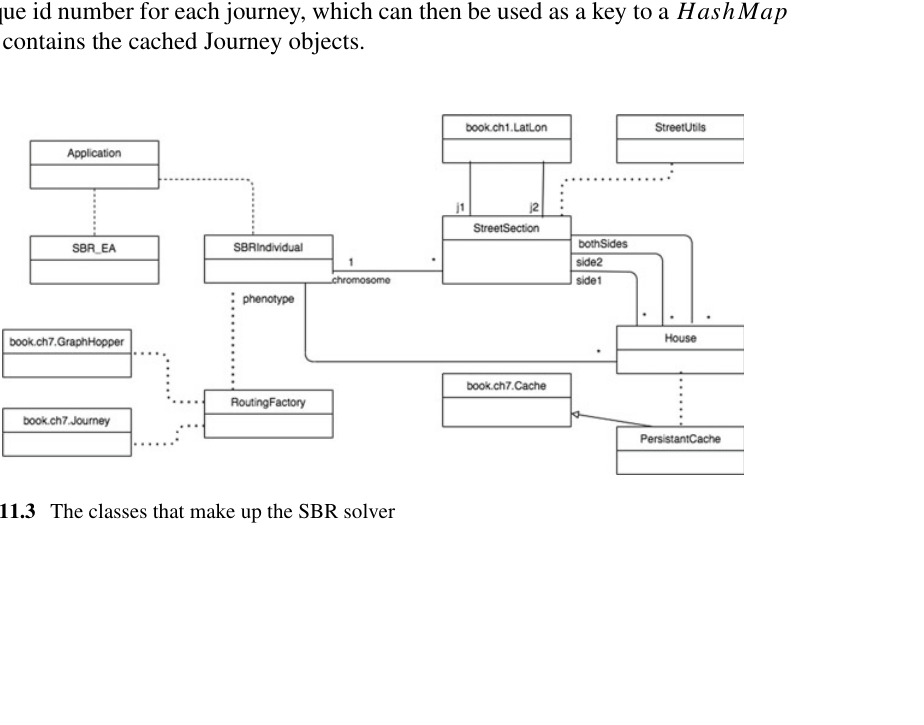
\includegraphics[width=0.72\linewidth]{fig_book_class_diagram.png}
  \end{center}

  The key components are:
  \begin{itemize}
    \item \textbf{PersistedCache} (the base class) --- stores pre-computed
          journey distances between delivery points.  When a distance between
          two points is requested, the cache is consulted first; only on a
          cache miss is the routing engine called.
    \item \textbf{RouteingEngine} --- wraps the GraphHopper library to
          compute walking distances between any two \texttt{LatLon} coordinates.
    \item \textbf{SBRChromosome} --- represents a candidate solution as an
          ordered list of \texttt{StreetSection} objects.
    \item \textbf{StreetSection} --- stores the two ordered lists of delivery
          addresses (side~1 and side~2), the two bounding junctions, and the
          pre-computed orderings for all delivery patterns.
  \end{itemize}

  \framebreak

  \textbf{Caching journeys with the Cantor Pairing Function.}
  A critical implementation challenge is how to look up cached walking
  distances quickly.  The cache stores \texttt{(start, end, distance)} triples
  in a Java \texttt{HashMap}.  The key for each entry must be a single integer
  that uniquely identifies the pair of street sections involved.

  The solution uses \textbf{Cantor's pairing function}.  Given two non-negative
  integers $x$ and $y$ (in our case, the hash codes of two street section
  objects), the Cantor pairing function returns a single unique integer $z$:

  \begin{block}{Cantor Pairing Formula}
    \[
      z = \tfrac{1}{2}(x + y)(x + y + 1) + y
    \]
    Here, $x$ is the hash code of the first street section (the starting point
    of the journey), $y$ is the hash code of the second street section (the
    ending point), and $z$ (the \emph{key}) is the unique integer assigned to
    the ordered pair $(x, y)$.
    The symbol $\frac{1}{2}$ means ordinary division by~2 (not integer
    division); since $(x+y)(x+y+1)$ is always even, $z$ is always a
    non-negative integer.
  \end{block}

  \textbf{Two important properties of Cantor pairing:}
  \begin{enumerate}
    \item For a given combination of $x$ and $y$, the same value $z$ is always
          returned --- so the same journey always maps to the same cache key.
    \item Each value of $z$ is associated with exactly one pair $(x, y)$ ---
          so there are never any collisions in the HashMap.
  \end{enumerate}

  \framebreak

  \begin{exampleblock}{Worked Example --- Cantor Pairing}
    Suppose street section A has hash code $x = 3$ and street section B has
    hash code $y = 5$.  Then:
    \[
      z = \tfrac{1}{2}(3 + 5)(3 + 5 + 1) + 5
        = \tfrac{1}{2} \times 8 \times 9 + 5
        = 36 + 5 = 41
    \]
    The journey from A to B is stored under key~41 in the HashMap.
    If we later need the distance from A to B again, we compute $z = 41$
    and look up \texttt{cache.get(41)} --- an $O(1)$ operation, far faster
    than calling the routing engine again.
  \end{exampleblock}

  \begin{center}
    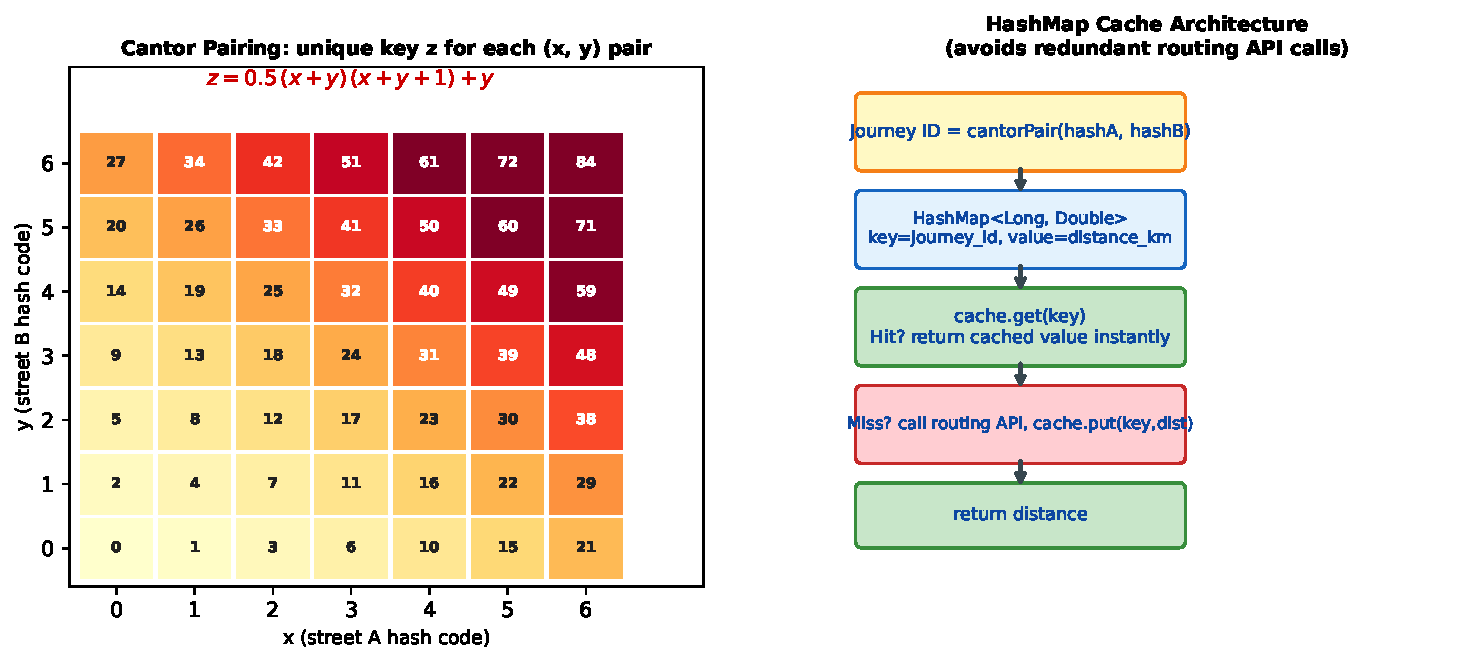
\includegraphics[width=0.75\linewidth]{fig_cantor_pairing.pdf}
  \end{center}

  The left panel shows the value of $z$ for all pairs $(x, y)$ up to $x=6,
  y=6$.  Each cell contains a unique integer --- note that no two cells share
  the same value.  The right panel shows the HashMap cache architecture:
  a journey key is computed, the HashMap is consulted, and only on a miss
  is the routing API called.

\end{frame}

\begin{frame}[fragile]{11.3 Implementation -- Java Code: Journey Cache}

  The listing below (Listing~11.1 in the book) shows the Java implementation
  of the journey distance cache.  This is one of the most performance-critical
  parts of the SBR implementation, because it is called once for every pair
  of consecutive street sections during every chromosome evaluation.

\begin{lstlisting}[style=java]
public double getJourneyDist(LatLon start, LatLon end, String mode) {
    // Compute a unique cache key from the hash codes of start and end
    long key = cantorPair(start.hashCode(), end.hashCode());

    // Try to retrieve a cached result first
    Double res = cache.get(key);
    if (res == null) {
        // Cache miss: call the routing engine to compute the distance
        options.put(RoutingEngine.OPTION_MODE, mode);
        res = router.findRoute(start, end, options).getDistanceKM();
        // Store the result for future reuse
        cache.put(key, res);
    }
    return res;
}

/*
 * Local cache backed by a HashMap.
 * key   = Cantor pair of the two endpoint hash codes (unique integer)
 * value = walking distance in kilometres
 */
private static HashMap<Long, Double> cache = new HashMap<Long, Double>();

private long cantorPair(long a, long b) {
    // Cantor's pairing function: maps (a, b) to a unique integer
    long result = (long) (0.5 * (a + b) * (a + b + 1) + b);
    return result;  // Return the unique key
}
\end{lstlisting}

  \textbf{Line-by-line explanation:}
  \begin{itemize}
    \item \textbf{Line 3:} The Cantor pair of the two hash codes forms the
          HashMap key.  Java's \texttt{hashCode()} method returns an integer
          representing each \texttt{LatLon} object.
    \item \textbf{Lines 5--11:} If the distance is in the cache, return it
          immediately without calling the router.  Otherwise, call the
          routing API, store the result, then return it.
    \item \textbf{Lines 18--22:} The \texttt{cantorPair} function implements
          the formula $z = 0.5(a+b)(a+b+1) + b$ exactly as described above.
          The cast to \texttt{long} ensures no integer overflow for large
          hash codes.
  \end{itemize}

\end{frame}

\begin{frame}[fragile]{11.3 Implementation -- Setting Up the Network in Code}

  To define the delivery area, the programmer creates a
  \textbf{StreetSection} object for each section, specifying the street name,
  the house numbers on each side, and the GPS coordinates of the two bounding
  junctions.

  The code listing below (Listing~11.2 in the book) shows how Greenbank
  Crescent in Edinburgh is added to the SBR chromosome:

\begin{lstlisting}[basicstyle=\ttfamily\tiny,frame=single,backgroundcolor=\color{gray!7},numbers=left,xleftmargin=1.5em]
chromo.addStreet(
    new StreetSection(
        "Greenbank Crescent, Edinburgh",
        new int[]{39,41,43,45,47,49,51,53,55,57,59,61,63,65,67,69},  // side 1
        new int[]{52,54,56,58,60,62,64,66,68,70,72,74,76,78,80,82},  // side 2
        new LatLon(55.9177482, -3.2166029),   // junction 1 GPS coordinates
        new LatLon(55.915377,  -3.216826)     // junction 2 GPS coordinates
    )
);
\end{lstlisting}

  \textbf{Reading this code:}
  \begin{itemize}
    \item The first argument is the human-readable street name (used for
          identification and debugging).
    \item The second and third arguments are arrays of house numbers for
          side~1 and side~2.  Even numbers are on one side, odd numbers on
          the other (as is conventional in UK addressing).
    \item The fourth and fifth arguments are the GPS coordinates (latitude,
          longitude) of the two junctions that bound this section of
          Greenbank Crescent.
  \end{itemize}

  \begin{block}{Latitude and Longitude (GPS Coordinates)}
    A \texttt{LatLon} object stores a pair of decimal numbers:
    the \emph{latitude} (north--south position, ranging from $-90^{\circ}$ to $+90^{\circ}$)
    and the \emph{longitude} (east--west position, ranging from $-180^{\circ}$ to
    $+180^{\circ}$).  For Edinburgh, latitude $\approx 55.9^{\circ}$ N and longitude
    $\approx -3.2^{\circ}$ (i.e.\ $3.2^{\circ}$ west of the Greenwich meridian).
    These coordinates are used by the routing engine to compute the actual
    walking distance between any two points.
  \end{block}

\end{frame}

%% =============================================================================
\section{11.4 Comparison with TSP}
%% =============================================================================

\begin{frame}[allowframebreaks]{11.4 Comparison with TSP -- The Case Study Area}

  To compare SBR-EA against a conventional TSP-EA, the authors use a real-world
  test case: the \textbf{Greenbank area of Edinburgh, Scotland}.  This is a
  residential district with a regular grid-like street layout, typical of
  urban postal delivery walks.

  \begin{center}
    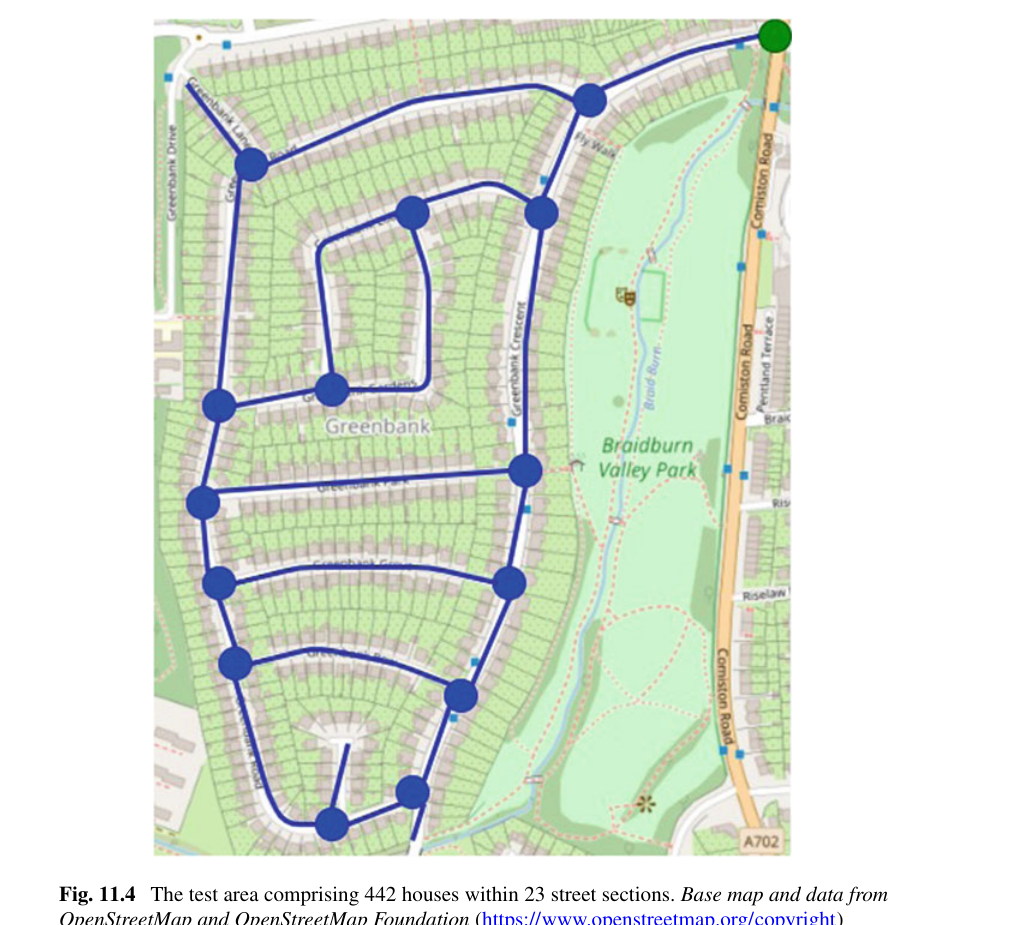
\includegraphics[width=0.65\linewidth]{fig_book_greenbank_area.png}
  \end{center}

  The test case consists of \textbf{442 delivery addresses} spread across
  \textbf{48 street sections} (some sections have only one side, some have
  both sides).

  \framebreak

  \textbf{The TSP formulation of the same problem:}
  The same 442 addresses can be formulated as a 442-city TSP problem, where
  each address is a ``city'' and the goal is to find the shortest tour visiting
  all of them.

  \begin{block}{Solution Space Size}
    For the TSP with 442 addresses, the solution space contains:
    \[
      \frac{442!}{2} = 5.487001 \times 10^{978} \text{ possible routes}
    \]
    The $442!$ counts all permutations of 442 addresses; dividing by 2
    removes duplicates caused by the fact that a route and its reverse have
    the same total length.  The number $5.487 \times 10^{978}$ is
    astronomically large --- for comparison, there are estimated to be
    only $10^{80}$ atoms in the observable universe.
  \end{block}

  \textbf{The SBR formulation of the same problem:}
  The SBR chromosome has 48 genes (street sections) plus some duplicates for
  double-sided sections.  Even if we count the approximate total number of
  orderings, the SBR search space is vastly smaller:
  \[
    48! \approx 1.24 \times 10^{61}
  \]
  This is still a very large number, but it is $10^{917}$ times smaller than
  the TSP space --- an enormous practical advantage.

  \begin{center}
    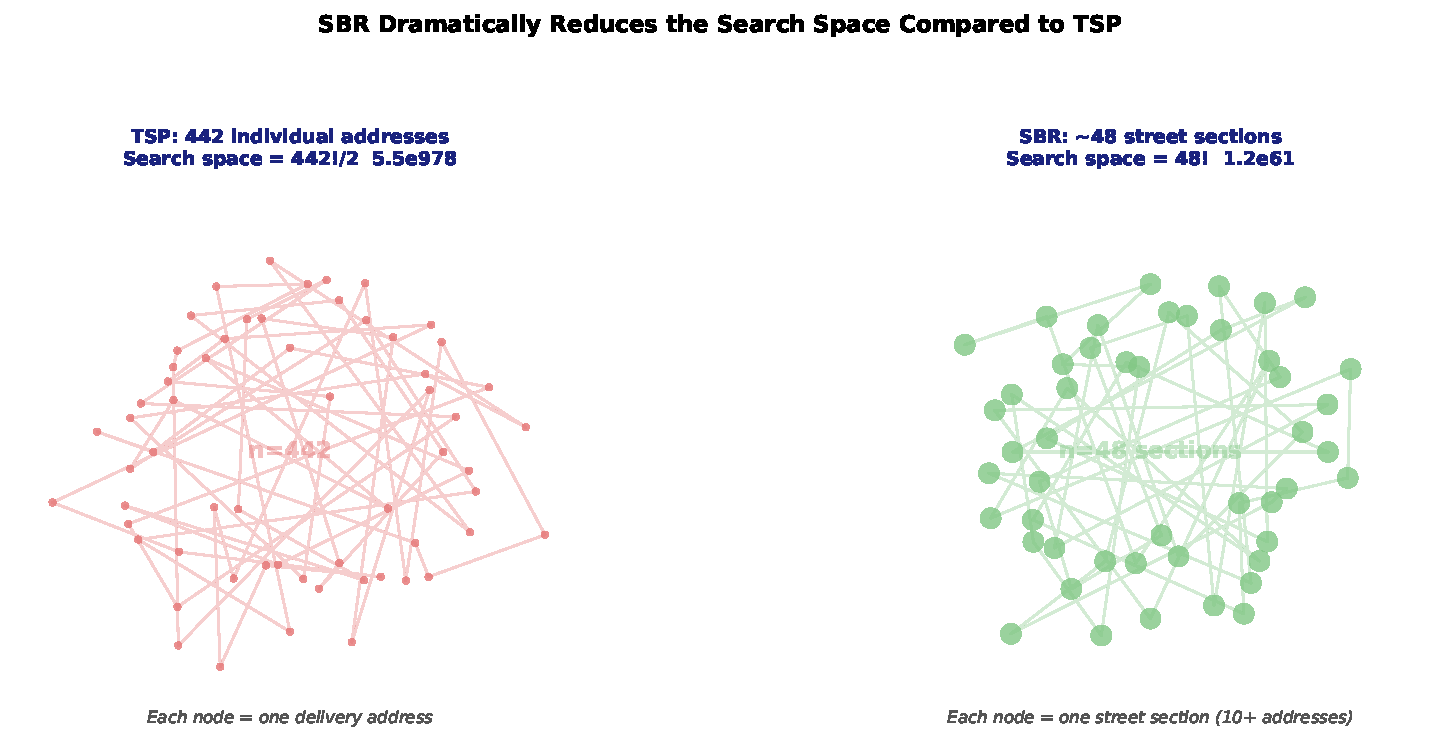
\includegraphics[width=0.72\linewidth]{fig_sbr_vs_tsp.pdf}
  \end{center}

  \framebreak

  \textbf{TSP fitness function.}  The fitness function for the TSP-EA is
  simply the \textbf{total route distance} from the start point to the end
  point, visiting all 442 addresses in order.  A standard nearest-neighbour
  heuristic initialises the population, and the Java EA implementation from
  the book's software repository is used for evaluation.

  \textbf{Results (Table~11.3).}
  Both EAs used a budget of \textbf{100,000 evaluations} and were run
  \textbf{10 independent times}.

  \begin{center}
    \begin{tabular}{lcccc}
      \toprule
      \textbf{Solver} & \textbf{Avg.\ time (s)} &
      \multicolumn{3}{c}{\textbf{Route distance (km)}} \\
      \cmidrule(lr){3-5}
       & & Min. & Avg. & Runs consistent? \\
      \midrule
      NN Heuristic & 20.3 & 10.2 & 10.2 & Yes (deterministic) \\
      SBR-EA       & \textbf{9.6}  & \textbf{6.8} & \textbf{7.7} & Variable \\
      TSP-EA       & 932.4 & 18.1 & 20.0 & Variable \\
      \bottomrule
    \end{tabular}
  \end{center}

  \begin{alertblock}{Headline Result}
    SBR-EA finds routes that are \textbf{24\% shorter than NN} and
    \textbf{about 2.6$\times$ shorter than TSP-EA}, while running approximately
    \textbf{100$\times$ faster} than TSP-EA.  Both EAs had the same evaluation
    budget, so this difference is entirely due to the smarter representation.
  \end{alertblock}

  \framebreak

  \begin{center}
    
\includegraphics[width=0.80\linewidth]{fig_results_comparison.pdf}
  \end{center}

  The left panel shows the route distance for each of the 10 runs for each
  solver.  The NN heuristic always produces the same 10.2~km route (it is
  deterministic).  SBR-EA consistently finds routes between 6.8~km and 8.3~km.
  TSP-EA, despite using 100 times more computation, finds routes between
  18~km and 22~km.

  The right panel shows the computation time on a log scale, making it clear
  that TSP-EA is over two orders of magnitude slower than SBR-EA.

\end{frame}

\begin{frame}[allowframebreaks]{11.4 Comparison with TSP -- Best Route Found}

  The best overall solution found by SBR-EA (6.8~km) is shown below on the
  real street map of the Greenbank area.  The red portion of the route indicates
  the final walk back to the depot after all deliveries are complete.

  \begin{center}
    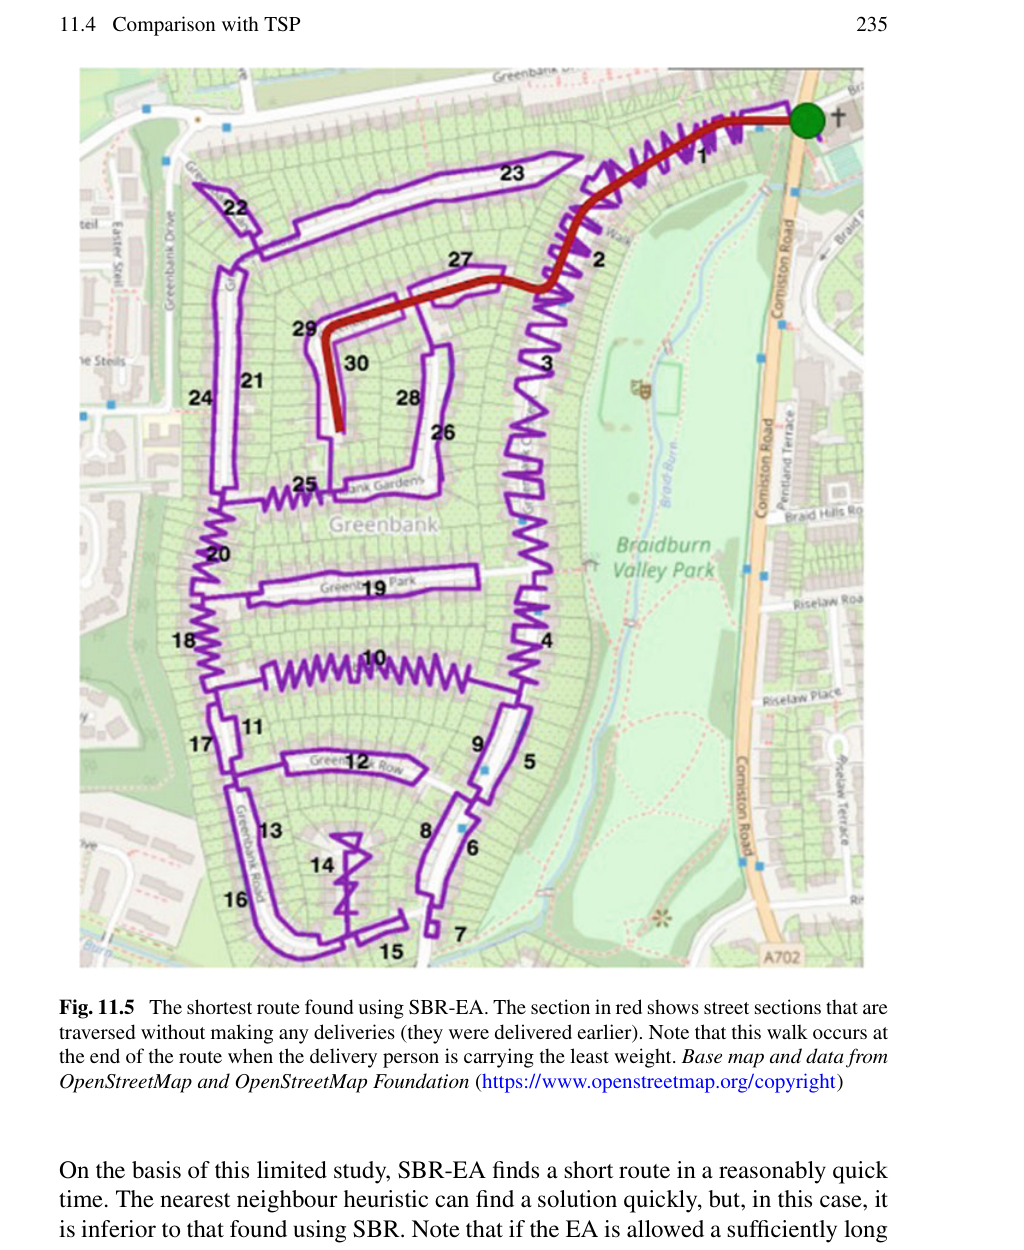
\includegraphics[width=0.72\linewidth]{fig_book_greenbank_route.png}
  \end{center}

  \textbf{Observations about the best SBR-EA route:}
  \begin{enumerate}
    \item The route encompasses continuous, uninterrupted deliveries until
          the very final walk back to the start.  The red section (return
          walk) occurs at the end when the worker is no longer carrying
          any load --- this is desirable from a physical-effort perspective.
    \item The initial street sections (numbers 1--4 in the route) are dealt
          with as \emph{double-sided} sections, meaning the worker delivers
          to both sides in a single sweep.  This keeps the undelivered load
          as low as possible early in the route, reducing the weighted
          return-walk penalty.
    \item The route has a broadly \emph{boustrophedon} (back-and-forth)
          structure, which is known to be near-optimal for grid-like street
          layouts.
  \end{enumerate}

  \begin{alertblock}{Why TSP-EA Performs So Poorly Here}
    TSP-EA's large search space means it cannot adequately explore good
    solutions within 100,000 evaluations.  It does not inherently group
    adjacent addresses together, so it wastes many moves crossing streets
    or doubling back.  SBR-EA, by construction, \emph{always} delivers all
    addresses in a section together, so its solutions are automatically
    sensible at the local level and the EA only needs to optimise the
    section ordering.
  \end{alertblock}

\end{frame}

%% =============================================================================
\section{11.5 Conclusions}
%% =============================================================================

\begin{frame}[allowframebreaks]{11.5 Conclusions}

  Street Based Routing is a \textbf{representation-and-decoder} combination
  tailored specifically to urban house-to-house delivery problems.  Rather
  than treating every individual address as an independent decision variable
  (as TSP does), SBR exploits the natural clustering of addresses into street
  sections and the connectivity of sections at junctions.

  \begin{block}{Summary of the SBR Approach}
    \begin{itemize}
      \item \textbf{Chromosome:} An ordered list of street sections (not
            individual addresses).  Double-sided sections appear twice.
      \item \textbf{Decoder:} Expands each gene into its pre-computed list
            of delivery addresses using one of three patterns (one-side,
            U-turn, cross-over) selected based on junction connectivity.
      \item \textbf{Pre-processing:} Optimal address orderings for all
            patterns are computed once at startup and cached; this makes
            each chromosome evaluation extremely fast.
      \item \textbf{Operators:} Mutation (random relocation, junction-based
            relocation, partner pairing) and recombination (junction-connected
            copying from two parents).
    \end{itemize}
  \end{block}

  \framebreak

  \textbf{Key advantages of SBR over TSP for urban delivery:}

  \begin{enumerate}
    \item \textbf{Massively reduced search space.}  For 442 addresses across
          48 sections, the SBR space ($48! \approx 10^{61}$) is $10^{917}$
          times smaller than the TSP space ($442!/2 \approx 10^{978}$).  The
          EA can therefore find much better solutions within the same
          evaluation budget.
    \item \textbf{Built-in domain knowledge.}  The SBR representation encodes
          the principle that adjacent addresses are delivered together.  This
          is always optimal locally, so the EA only needs to optimise global
          section ordering.
    \item \textbf{Speed.}  The combination of a smaller search space and
          cached address orderings makes SBR-EA approximately 100$\times$
          faster than TSP-EA on the Greenbank test case.
  \end{enumerate}

  \textbf{Limitations and honest caveats:}

  \begin{itemize}
    \item SBR \emph{cannot represent} solutions that split a street section's
          addresses across different parts of the route.  A pure TSP could
          theoretically find such solutions if they happened to be shorter.
          The authors acknowledge this, but argue that in practice the speed
          advantage of SBR outweighs the possibility of missing such exotic
          solutions.
    \item The comparison in this chapter is intentionally limited in scope
          (one study area, one budget, 10 runs).  Larger studies could
          give more robust statistical conclusions.
    \item The implementation uses a routing engine (GraphHopper) to compute
          walking distances.  Any system that cannot call a routing API would
          need to fall back to Euclidean or Manhattan distances.
  \end{itemize}

  \framebreak

  \begin{alertblock}{The Big Takeaway}
    Domain knowledge, when correctly encoded into the chromosome representation
    and decoding process, can reduce the effective search space by many orders
    of magnitude and produce dramatically better solutions within the same
    computational budget.  SBR is a prime example of this principle: by
    exploiting the structure of urban streets, it finds routes that are both
    shorter and found faster than a general-purpose TSP approach.
  \end{alertblock}

  \textbf{Broader applicability.}  The SBR principle generalises to any
  problem where deliveries or visits cluster naturally into groups:
  political canvassing, census data collection, utility meter reading,
  and any other house-to-house operation in urban areas.  The key requirement
  is that the groups (street sections) be well-defined, bounded by identifiable
  transition points (junctions), and that within-group ordering can be
  pre-optimised.

  \begin{block}{References}
    \begin{footnotesize}
    \begin{itemize}
      \item Urquhart, N., B.\ Paechter, and K.\ Chisholm. 2001.
            Street-Based Routing Using an Evolutionary Algorithm.
            In \emph{Applications of Evolutionary Computing}, ed.\ E.J.W.\ Boers,
            495--504. Springer.
      \item Urquhart, Neil. 2002.
            \emph{Solving a Real-World Routing Problem using Evolutionary
            Algorithms and Agents}, PhD Thesis, Edinburgh Napier University.
      \item Pigeon, Steven. n.d.\ Pairing Function. \emph{From MathWorld -- A
            Wolfram Web Resource}.
            \url{https://mathworld.wolfram.com/PairingFunction.html}
    \end{itemize}
    \end{footnotesize}
  \end{block}

\end{frame}

%% =============================================================================
%% APPENDIX: Worked Numerical Examples
%% =============================================================================

\appendix
\section{Appendix: Worked Numerical Examples}

\begin{frame}[allowframebreaks]{Appendix A -- Worked Example: Full SBR Decoding}

  This appendix walks through a complete, concrete decoding of a small
  SBR chromosome to show every step of Algorithm~22.

  \textbf{Setup.}  Suppose our delivery area has three street sections:
  \begin{center}
    \begin{tabular}{lll}
      \toprule
      Section & Addresses side~1 & Addresses side~2 \\
      \midrule
      \texttt{AlphaRd1}   & 1, 3, 5, 7, 9   & 2, 4, 6, 8, 10 \\
      \texttt{BetaLane1}  & 11, 13, 15      & 12, 14, 16 \\
      \texttt{GammaAv1}   & 17, 19, 21      & --- (one side only) \\
      \bottomrule
    \end{tabular}
  \end{center}
  (\texttt{Alpha} and \texttt{Beta} are double-sided; \texttt{Gamma} is
  one-sided.)  The depot is at junction~J0.  Walking distances between
  consecutive houses within a section are 30~m each; distances between
  junctions and neighbouring houses are 20~m; distance from the depot
  to the first house on each section is 100~m.

  \textbf{Chromosome to decode:}
  \[
    [\texttt{GammaAv1},\ \texttt{AlphaRd1},\ \texttt{AlphaRd1},\ \texttt{BetaLane1},\ \texttt{BetaLane1}]
  \]
  Note: \texttt{AlphaRd1} and \texttt{BetaLane1} each appear twice (both sides).

  \framebreak

  \textbf{Step-by-step decoding:}

  \textbf{Gene 1 --- \texttt{GammaAv1} (single-sided):}
  \begin{itemize}
    \item Previous location: depot (J0).
    \item Start junction: the junction of \texttt{GammaAv1} nearest to J0.
      Suppose this is junction~J1.
    \item One-side pattern: deliver addresses 17, 19, 21 in order from J1
      to J2.  Walking distance within section: $3 \times 30 = 90$~m.
    \item Distance from depot to first address (\#17): 100~m.
    \item Subtotal so far: $100 + 90 = 190$~m.
  \end{itemize}

  \textbf{Genes 2 and 3 --- \texttt{AlphaRd1} (double-sided, adjacent):}
  \begin{itemize}
    \item Gene 2 equals Gene 3, so \texttt{doubleSided = true}.
    \item U-turn pattern: deliver side~1 (1, 3, 5, 7, 9) walking J1 to J3;
      then deliver side~2 (10, 8, 6, 4, 2) walking back J3 to J1.
    \item Walking distance side~1: $4 \times 30 = 120$~m.  U-turn: 0~m extra.
      Walking distance side~2: $4 \times 30 = 120$~m.
    \item Walking from end of \texttt{Gamma} to start of \texttt{Alpha}:
      suppose 80~m (between J2 and J1).
    \item Subtotal this section: $80 + 120 + 120 = 320$~m.
    \item Cumulative total: $190 + 320 = 510$~m.
  \end{itemize}

  \textbf{Genes 4 and 5 --- \texttt{BetaLane1} (double-sided, adjacent):}
  \begin{itemize}
    \item Same logic: U-turn pattern; 3 houses per side.
    \item Walking side~1: $2 \times 30 = 60$~m; side~2: $2 \times 30 = 60$~m.
    \item Walking from \texttt{Alpha} to \texttt{Beta}: suppose 90~m.
    \item Subtotal: $90 + 60 + 60 = 210$~m.
    \item Cumulative total: $510 + 210 = 720$~m.
  \end{itemize}

  \textbf{Return walk to depot:}
  Suppose 150~m from the last address on \texttt{Beta} back to the depot.
  At this point \texttt{deliveriesLeft} = 0 (all addresses delivered),
  so the penalty term is $150 \times 0 = 0$~m extra.

  \textbf{Total route distance: $720 + 150 = 870$~m.}

  \begin{alertblock}{Note on the Penalty Term}
    The penalty term $\mathtt{walkingDist}(lastDel, end) \times
    \mathtt{deliveriesLeft}$ is zero when all deliveries are made before
    the return walk (as here).  It becomes large when deliveries are spread
    unevenly, forcing a long return trip while still carrying packages.
    This steers the EA towards solutions that front-load deliveries.
  \end{alertblock}

\end{frame}

\begin{frame}[allowframebreaks]{Appendix B -- Worked Example: Cantor Pairing in the Cache}

  This example traces the cache behaviour during a small EA evaluation run
  to illustrate how Cantor pairing prevents redundant routing calls.

  \textbf{Setup.}  Suppose the routing engine takes 200~ms to compute each
  walking distance.  Our EA evaluates 10,000 chromosomes.  Each chromosome
  has on average 30 gene-to-gene transitions.  Without caching, total routing
  calls = $10,000 \times 30 = 300,000$, taking $300,000 \times 0.2$~s $=
  60,000$~s $\approx$ 17 hours.

  \textbf{With caching.}  For a delivery area with 48 street sections, there
  are at most $48 \times 48 = 2,304$ unique ordered pairs (section~A followed
  by section~B).  After the cache is ``warm'' (all pairs seen at least once),
  every subsequent routing query is a HashMap look-up taking $\approx 0.001$~ms.

  \textbf{Warm-up phase:} at most 2,304 routing calls, costing
  $2,304 \times 0.2 = 461$~s $\approx 8$~minutes.

  \textbf{Steady-state phase:} all 10,000 chromosomes evaluated with only
  HashMap look-ups, costing essentially zero routing engine time.

  \begin{exampleblock}{Cantor Key Computation for a Specific Pair}
    Section \texttt{Greenbank Crescent N} has hash code $x = 12345$.
    Section \texttt{Greenbank Drive E} has hash code $y = 67890$.
    \begin{align*}
      z &= \tfrac{1}{2}(12345 + 67890)(12345 + 67890 + 1) + 67890 \\
        &= \tfrac{1}{2} \times 80235 \times 80236 + 67890 \\
        &= \tfrac{1}{2} \times 6{,}437,823,060 + 67890 \\
        &= 3{,}218{,}911{,}530 + 67890 \\
        &= 3{,}218{,}979{,}420
    \end{align*}
    The walking distance from \texttt{GreenBank Crescent N} to
    \texttt{Greenbank Drive E} is stored in the HashMap under the key
    $3{,}218{,}979{,}420$.  This is a 32-bit integer that fits comfortably
    in a Java \texttt{long}.
  \end{exampleblock}

\end{frame}

\begin{frame}[allowframebreaks]{Appendix C -- Solution Space Size: Numbers in Perspective}

  Understanding just how large the TSP solution space is helps motivate the
  need for SBR.  The following table puts the numbers in context.

  \begin{center}
    \begin{tabular}{lrl}
      \toprule
      \textbf{Quantity} & \textbf{Approximate value} & \textbf{Notes} \\
      \midrule
      Atoms in observable universe & $10^{80}$ & \\
      TSP solutions for 442 addresses & $5.5 \times 10^{978}$ &
            $= 442!/2$ \\
      SBR solutions for 48 sections  & $1.2 \times 10^{61}$ &
            $= 48!$ \\
      Ratio (TSP / SBR)              & $\approx 10^{917}$ &
            SBR space is this many times smaller \\
      TSP solutions for 20 cities    & $6.1 \times 10^{16}$ &
            Still 61 quadrillion routes \\
      TSP solutions for 10 cities    & $1.8 \times 10^{5}$ &
            181,440 --- searchable by brute force \\
      \bottomrule
    \end{tabular}
  \end{center}

  \textbf{A physical analogy.}  Imagine you have a deck of 442 playing cards
  (with additional cards added beyond the standard 52).  The number of ways to
  shuffle those cards is $442! / 2 \approx 5.5 \times 10^{978}$.  If you could
  shuffle the deck once per nanosecond and had been doing so since the Big Bang
  ($\approx 13.8$ billion years ago), you would have explored approximately
  $4.4 \times 10^{26}$ arrangements --- a number so small compared to $10^{978}$
  that you would not even have made a dent in the full space.

  This illustrates why evolutionary algorithms with smart representations are
  not merely a convenience: they are a necessity for practical combinatorial
  optimisation at realistic problem sizes.

\end{frame}

\end{document}
